\normaltrue
\correctionfalse

%\UPSTIidClasse{12} % 11 sup, 12 spé
%\newcommand{\UPSTIidClasse}{12}

\exer{Automate d’exploration de l’hémostase $\star$ \label{DYN:02:C2:09:1D:61}}
\setcounter{question}{0}\marginnote{\xpComp{DYN}{01}}%\UPSTIcompetence[2]{C2-09}
\index{Compétence C2-09}\index{Compétence DYN-01}
\index{Principe fondamental de la dynamique}
\index{PFD}
%\index{Mécanisme à 1 rotation}
\index{Automate d’exploration de l’hémostase}
\ifcorrection
\else
\marginnote{\textbf{Pas de corrigé pour cet exercice.}}
\fi

\ifprof
\else
Afin de valider le choix des moteurs, on étudie le déplacement sur l’axe $\vect{x}$.% qui est le plus grand. 
On note $V_x$ la vitesse selon cet axe.
On rappelle que la distance maximum à parcourir est $x_M^{\text{max}} = \SI{550}{mm}$ en 1 seconde.
La loi de commande sur chaque axe est définie par un trapèze de vitesse (\autoref{61_01})
avec les temps d’accélération et de décélération ($T_a$) identiques. De plus, les moteurs se mettent en route et s’arrêtent en
même temps. $T$ est la durée totale du déplacement. Nous allons chercher à optimiser cette loi de commande de sorte
que le moteur fournisse une puissance instantanée minimale.

\begin{figure}[H]
\centering
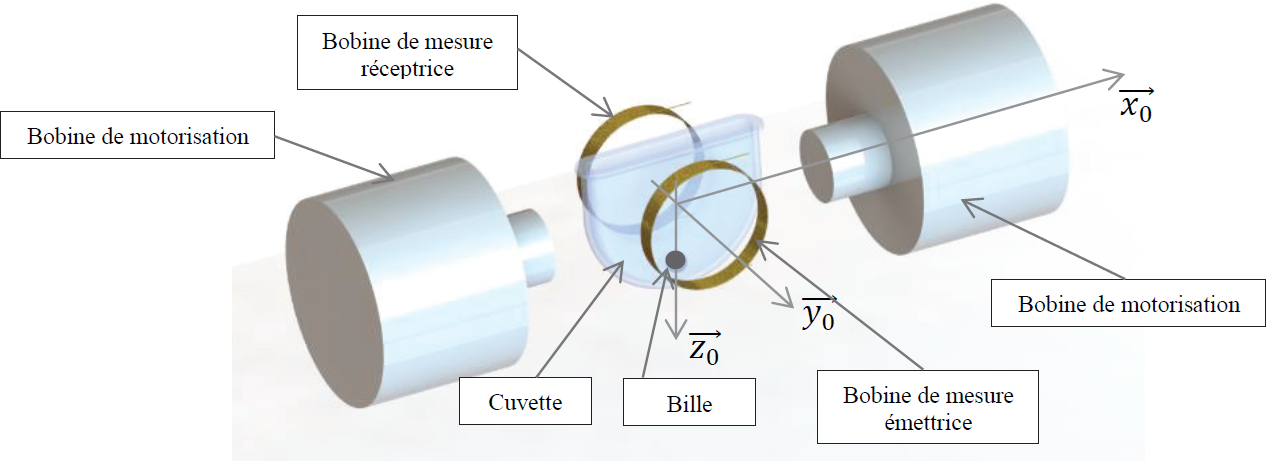
\includegraphics[width=.8\linewidth]{61_01}
\caption{\label{61_01} Loi de commande de vitesse en trapèze}
\end{figure}

Le modèle de calcul pour cette commande d’axe est le suivant :
\begin{itemize}
\item le mouvement de rotation du moteur (vitesse $\omega_m^x$) est transformé en mouvement de translation (vitesse $V^x$) ;
\item le rapport de transmission de la chaîne cinématique est $\lambda = \dfrac{V^x}{\omega_m^x}$;
\item la distance à parcourir est $x_M^{\text{max}}$;
\item l’inertie équivalente de l’ensemble des pièces en mouvement ramenée à l’arbre moteur est $J_e$;
\item les frottements et la pesanteur sont négligés, il n’y a donc pas de couple résistant.
\end{itemize}
\fi
\question{Exprimer la vitesse maximale $V_M^x$ en fonction de $x_M^{\text{max}}$, $T$ et $T_a$.}
\ifprof
La distance  $x_M^{\text{max}}$ correspond à l'aire sous le courbe de la loi de commande de vitesse.
On a alors 
 $x_M^{\text{max}} = \left(T-T_a\right)V_M^x$ 
 $ \Longleftrightarrow V_M^x=\dfrac{x_M^{\text{max}}}{T-T_a}$. 
\else
\fi

\question{Par application du théorème de l’énergie cinétique sur l’ensemble des pièces en mouvement,
exprimer le couple moteur $C_m$ en fonction de $V_x$, $T_a$, $J_e$ et $\lambda$ durant les trois phases du
mouvement.}
\ifprof
\begin{itemize}
\item Expression de l'énerige cinétique : $\ec{E}{0}=\dfrac{1}{2}J_e (\omega_m^x)^2$.
\item Puissance intérieure : $\mathcal{P}_{\text{int}}(E)=0$.
\item Puissance extérieure : $\mathcal{P}_{\text{ext}}(E)=C_m\omega_m^x$.
\item Application du TEC : $J_e \omega_m^x \dot{\omega}_m^x = C_m\omega_m^x$ soit $J_e  \dot{\omega}_m^x = C_m$.
\end{itemize}
\vspace{.25cm}

On a alors sur chacune des phases : 

\begin{itemize}
\item Phase 1 : $C_m=J_e  \dot{\omega}_m^x$ avec $\dot{\omega}_m^x = \dot{V_M}^x /  \lambda= \dfrac{V_M^x}{ \lambda T_a}$ et $C_m = J_e \dfrac{V_M^x}{\lambda T_a}$.
\item Phase 2 : $C_m=0$.
\item Phase 3 : $C_m = - J_e  \dfrac{V_M^x}{\lambda T_a}$.
\end{itemize}

\else
\fi

\question{Préciser à quel(s) instant(s) $t$ la puissance fournie par le moteur est maximale ($P_{\text{max}}$)}.
\ifprof
\else
\fi

\question{Exprimer cette puissance $P_{\text{max}}$ en fonction de $V_M^x$, $\lambda$, $J_e$, et $T_a$.}
\ifprof
$P_{\text{max}} = J_e \dfrac{V_M^x}{\lambda T_a}  {\omega}_m^x =J_e \dfrac{(V_M^x)^2}{\lambda^2 T_a}$.
\else
\fi

\question{Donner alors l’expression de $P_{\text{max}}$ en fonction de $x_M^{\text{max}}$, $\lambda$, $J_e$, et $T_a$.}
\ifprof
On a alors 
$P_{\text{max}} =J_e \dfrac{\left({x_M^{\text{max}}}\right)^2}{\lambda^2 \left({T-T_a}\right)^2 T_a}$.
\else
\fi

\question{À partir de cette expression, montrer que $P_{\text{max}}$ est minimale pour un réglage du
temps d’accélération $T_a$ tel que $T_a=\dfrac{T}{3}$.}
\ifprof
On résout $\dfrac{\dd P_{\text{max}}}{\dd T_a} = 0$ et on cherche la valeur de $T_a$ pour laquelle 
$P_{\text{max}}$ est minimale.

\else
\fi

\ifprof
\else
Pour cette nouvelle commande avec $T_a=\dfrac{T}{3}$, on cherche à valider le choix du moteur en étudiant le
déplacement maximum suivant $\vect{x}$. Les caractéristiques de la chaîne cinématique sont :
\begin{itemize}
\item vitesse maximale du moteur : $N_{\text{max}}^{\text{mot}}=\SI{4150}{tr.min^{-1}}$;
\item rapport de réduction du réducteur $k=\dfrac{1}{10}$;
\item rayon de poulie $R_p= \SI{20}{mm}$.
\end{itemize}
\fi

\question{Déterminer la vitesse de rotation maximum $\omega^x_{\text{max}}$ que doit atteindre le moteur. Le
choix de celui-ci est-il validé ?}
\ifprof
On a  $V_M^x=\dfrac{x_M^{\text{max}}}{T-T_a}$. D'autre part, 
$V_M^x = \omega_M^x  k R_p $ soit $\omega_M^x  = \dfrac{V_M^x}{ k R_p} =  \dfrac{{x_M^{\text{max}}}}{ k R_p\left({T-T_a} \right)} $.

AN : $\omega_M^x  = \dfrac{550\times 10^{-3}}{ 0,1 \times 20 \times 10^{-3} \left(1-1/3 \right)} $
$ =  \dfrac{550\times 3}{ 4}= \SI{412,5}{rad.s^{-1}} $ soit \SI{3941}{tr.min^{-1}}.

Cette valeur est bien compatible avec la vitesse du moteur.
\else
\fi


\ifprof
\else

\marginnote{Corrigé voir \ref{DYN:02:C2:09:1D:61}.}

\fi